%!TeX root = Chapter_Data2
\documentclass[../../CompleteThesis2/Complete_2ndDraft]{subfiles}
%\graphicspath{{../../Figures/}}
\begin{document}

\section[Volcanic Horizons][Volcanic Horizons]{Determining Time of Volcanic Material Deposition}
\label{Sec:Data_VolcanicHorizons}

\subsection[Corrected Depth]{Corrected Depth Estimate}
\label{Subsec:Data_VolcanicHorizons_CorrDepthEst}

\subsection[Gaussian Distribution]{Gaussian Distribution}
\label{Subsec:Data_VolcanicHorizons_GaussDist}

\section[Selection][Selection]{Selection of Isotopic Data}
\label{Sec:Data_Selection}

The method developed in this project is very general and can hopefully be used for information reconstruction and diffusion length estimation in a great number of different ice cores. But to develop a general algorithm one must first test it on specific data sets. I chose to focus mainly on a number of shallow ice cores, the Alphabet cores near the Greenlandic ice core Crete, and especially on the core drilled at Site A, see Figure \ref{Alphabet_Map} for location of the different cores examined.

\subsection[AWI B-cores]{AWI B-cores: Core B23}
\label{Subsec:Data_Selection_Bcores}
\todo{DATA: Make spatial map of B-cores locations.}
Before choosing to focus mainly on the Alphabet cores, some time was spend on examining a number of cores of length between 100-175 m drilled during the North Greenland Transverse (NGT) between 1993 and 1995 in northern Greenland, from now on referred to as the AWI (Alfred-Wegener-Institut) B-cores, \cite[Weissbach et al. 2016]{Weissbach2016}. These were primarily chosen due to their great spatial coverage of an area of roughly 10 \% of the Greenland ice sheet. This could have proven very useful for using the method developed here to estimate a spatial-temporal map of the covered area in the period between the eruptions of Laki and Tambora. Unfortunately the data from the AWI B-cores where not of high enough quality to meet the requirements of the following data analysis. Of the twelve AWI B cores available, only seven had corresponding electrical conductivity measurements with recognizable Laki and Tambora signals. Out of these seven only three were of adequate quality and resolution to subsequently be analyzed, see Appendix \ref{App:Data_AWI}. The $\delta^{18}$O and electrical conductivity profiles of one of the three high-quality cores from the NGT can be seen in Figure \ref{fig:B23_ECMd18O_combo}.

\begin{figure}[h]
	\centering
	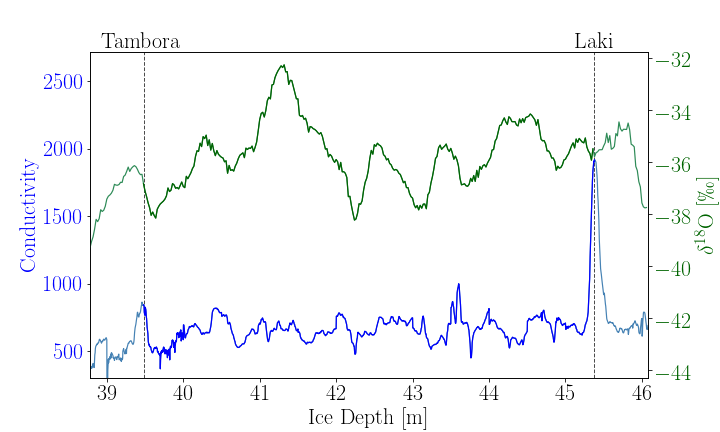
\includegraphics[width=0.8\textwidth]{B23_ECMd18O_combo.png}
	\caption[]{$\delta^{18}$O and conductivity profile of the AWI B-core B23. The dashed lines represent the suggested locations of the Laki and Tambora eruptions as matched in \cite[Weissbach et al. 2016]{Weissbach2016}}
	\label{fig:B23_ECMd18O_combo}
\end{figure}


\subsection[Crete Area][Crete Area]{Crete and Surrounding Alphabet Cores: Site A}
\label{Subsec:Data_Selection_Alhabet}
\todo{DATA: Make map of Alphabet core locations.}
The cores drilled in 1984-85 around the Crête core consist of the 400 m Crête core obtained in 1974 \cite{bibid} and eight shallow cores of varying length, between 25 m and 130 m, drilled in the Crête vicinity with a spatial coverage of 150 $\times$ 150 km, \cite[Clausen, Gundestrup, Johnsen 1988]{Clausen1988}.
Only two cores were not of use for this project, due to their shallow maximal depth, Site C and Site F, and the remaining seven cores, along with the Crête core, make up the eight cores in focus of this project. They are all well-documented, \cite[Clausen \& Hammer, 1988]{ClausenHammer1988}, \cite[Clausen, Gundestrup, Johnsen 1988]{Clausen1988}, and of high resolution making them ideal for the data and signal analysis used in the scope of this thesis. In Figures \ref{fig:SiteA__ECM_d18O_full.png}, \ref{fig:SiteA_d18OInsert}, \ref{fig:SiteA_ECMInsert} and \ref{fig:SiteA_ECMd18O_combo} the $\delta^{18}$O and conductivity data from the single ice core Site A can be seen, both the core in full length, \ref{fig:SiteA__ECM_d18O_full.png} and with corresponding zoom-ins on the matched Laki to Tambora depth series, Figures \ref{fig:SiteA_d18OInsert}, \ref{fig:SiteA_ECMInsert} and \ref{fig:SiteA_ECMd18O_combo}.
\begin{figure}[h]
	\centering
	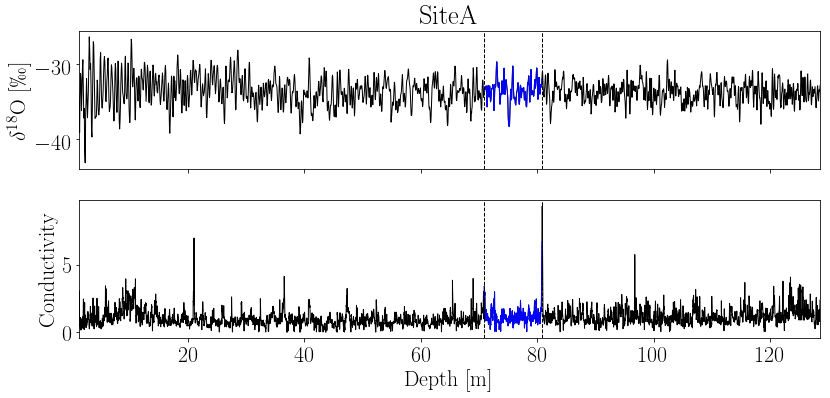
\includegraphics[width=\textwidth]{SiteA_ECM_d18O_full.png}
	\caption[]{}
	\label{fig:SiteA__ECM_d18O_full.png}
\end{figure}

\begin{figure}[h]
	\centering
	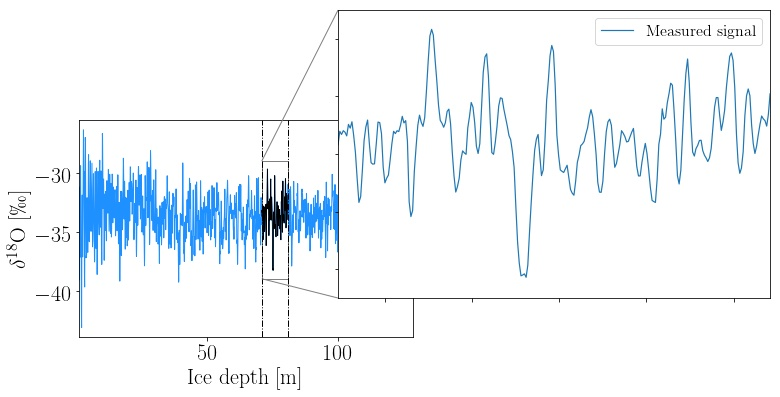
\includegraphics[width=\textwidth]{SiteA_d18OInsert.jpg}
	\caption[]{}
	\label{fig:SiteA_d18OInsert}
\end{figure}

\begin{figure}[h]
	\centering
	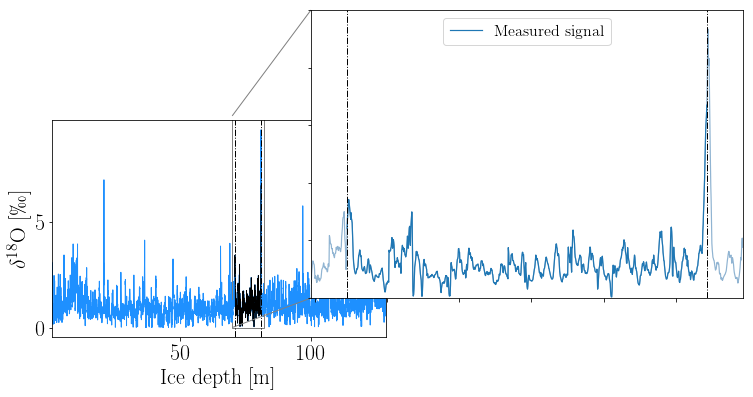
\includegraphics[width=\textwidth]{SiteA_ECMInsert.png}
	\caption[]{}
	\label{fig:SiteA_ECMInsert}
\end{figure}

\begin{figure}[h]
	\centering
	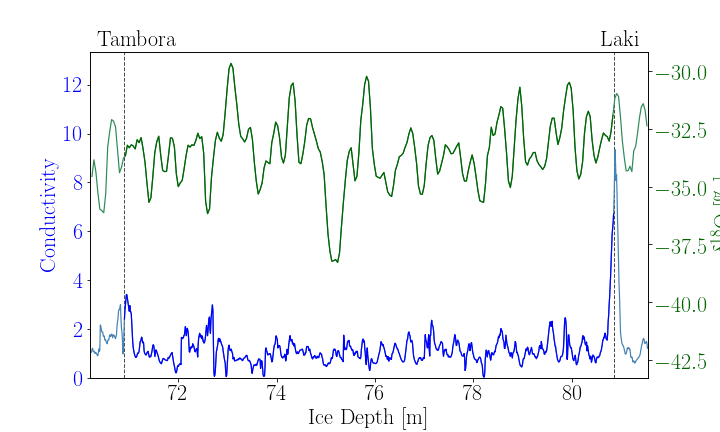
\includegraphics[width=0.8\textwidth]{SiteA_ECMd18O_combo.png}
	\caption[]{}
	\label{fig:SiteA_ECMd18O_combo}
\end{figure}

\subsubsection[Data Specifications][Data Specifications]{Data Specifications}
\label{Subsubsec:Data_Selection_Alhabet_Specifications}
Example of one cores specification. \todo{DATA-ALPHABET-SPECS: Put rest of specifications in appendix.}






\end{document}